%!TEX encoding = UTF-8 Unicode
%!TEX root = manuscript.tex
%
% ------------------------------------------ 
%     ICIP/ICASSP 向け LaTeX テンプレート
% ------------------------------------------ 
% 
% ・ ICIP / ICASSP 向けの Author Kit 
%
\documentclass{article}
\usepackage{spconf}
%!TEX encoding = UTF-8 Unicode
%
% 卒論 / 修論用 プリアンブル
%

%% フォント
\usepackage{lmodern}
\usepackage[scale=0.95]{tgheros}
\usepackage{textcomp}
\usepackage[scaled=0.85]{beramono}
\usepackage[T1]{fontenc}

%% パッケージ
\usepackage[cmex10]{amsmath}
\usepackage{amssymb,amsfonts,mathtools,bm}

\usepackage{graphicx,color}
\usepackage[table]{xcolor}

\usepackage[pdfborder={0 0 0}]{hyperref}
\usepackage{pxjahyper}

% caption のコロン「図4.4: キャプション」を「図4.4 キャプション」に直す
\usepackage[labelsep=quad,compatibility=false]{caption}
\usepackage[belowskip=1.2em]{subcaption}

\usepackage{cite,url,array,makecell}
\usepackage{algorithm,algorithmic}

% 数学コマンドの補完
\DeclareMathOperator*{\sinc}{sinc}
\DeclareMathOperator*{\prox}{prox}
\DeclareMathOperator*{\argmin}{argmin}
\DeclareMathOperator*{\argmax}{argmax}

% 参考文献表示スタイルを変更
\bibliographystyle{sieicej}

% 赤色を少し暗くする
\definecolor{red}{rgb}{0.75,0,0}

\makeatletter
   % アルゴリズム図キャプションの表記を「Algorithm」→「アルゴリズム」に
   \renewcommand{\ALG@name}{アルゴリズム}
\makeatother

% 修正箇所に色付けするコマンド
%
% ・ コマンド版
%   \fixed{修正箇所}
%
% ・ 環境版
%   \begin{fixedregion}
%      修正箇所
%   \end{fixedregion}
\newcommand{\fixed}[1]{#1} 
\newenvironment{fixedregion}{\ignorespaces}{\ignorespacesafterend}
% 下の 2 行をコメントアウトすることで色付けを無効化します
\renewcommand{\fixed}[1]{\textcolor{red}{#1}}
\renewenvironment{fixedregion}{\protect\leavevmode\color{red}\ignorespaces}{\ignorespacesafterend}

% 強調
\newcommand{\strong}[1]{\textcolor{red}{\textbf{#1}}}



%% \title : 一般の LaTeX 文書と同じ
\title{ICIP/ICASSP Paper Template}

%% \author の代わりに \name, \address を使う
\name{Takanori Fujisawa, Masaaki Ikehara}
\address{EEE Dept., Keio Univ., Yokohama, Kanagawa 223-8522, Japan\\
         \url{{fujisawa, ikehara}@tkhm.elec.keio.ac.jp}}

\begin{document}
%% 文字サイズを 9pt に (スペースが余りすぎるようならコメントアウトする)
\ninept

\maketitle

%% 概要
\begin{abstract}
The abstract should appear at the top of the left-hand column of text, about
0.5 inch (12 mm) below the title area and no more than 3.125 inches (80 mm) in
length.  Leave a 0.5 inch (12 mm) space between the end of the abstract and the
beginning of the main text.  The abstract should contain about 100 to 150
words, and should be identical to the abstract text submitted electronically
along with the paper cover sheet.  All manuscripts must be in English, printed
in black ink.
\end{abstract}

%% キーワード
\begin{keywords}
LaTeX, Template
\end{keywords}

\section{Introduction}
These guidelines include complete descriptions of the fonts, spacing,
and related information for producing your proceedings manuscripts
% 引用は複数まとめて \cite に入れられる
\cite{Example-Proceedings,Example-Article}.
Please follow them and if you have any questions, 
direct them to Conference Management Services, Inc.: 
Phone +1-979-846-6800 or email to \url{ip17@securecms.com}.

\section{MAJOR HEADINGS}
\label{sec:majhead}

Major headings, for example, ``1. Introduction'', should appear in all capital
letters, bold face if possible, centered in the column, with one blank line
before, and one blank line after. Use a period (``.'') after the heading number,
not a colon.

\subsection{Subheadings}
\label{ssec:subhead}

Subheadings should appear in lower case (initial word capitalized) in
boldface.  They should start at the left margin on a separate line.
 
\subsubsection{Sub-subheadings}
\label{sssec:subsubhead}

Sub-subheadings, as in this paragraph, are discouraged. However, if you
must use them, they should appear in lower case (initial word
capitalized) and start at the left margin on a separate line, with paragraph
text beginning on the following line.  They should be in italics.

\section{Formatting your paper}
\label{sec:format}
All printed material, including text, illustrations, and charts, must be kept
within a print area of 7 inches (178 mm) wide by 9 inches (229 mm) high. Do
not write or print anything outside the print area. The top margin must be 1
inch (25 mm), except for the title page, and the left margin must be 0.75 inch
(19 mm).  All \emph{text} must be in a two-column format. Columns are to be 3.39
inches (86 mm) wide, with a 0.24 inch (6 mm) space between them. Text must be
fully justified.
% 数式,セクションの頭に数式を入れると余白が変なことになるので注意
\begin{equation}
  2 \pi \phi_i (\bm r_i) =
    + \frac{\varepsilon_1}{\varepsilon_2}
      \sum_{j=1}^{N_p} (\bm r_j)
        \sqrt{ 
          \int_{\Gamma_j} 
            \frac{e^{-\kappa | \bm r_i - \bm r^\prime | }}
                 { | \bm r_i - \bm r^\prime | } 
              d\Gamma^\prime }
\end{equation}


\section{Page Title Section}
\label{sec:pagestyle}

The paper title (on the first page) should begin 1.38 inches (35 mm) from the
top edge of the page, centered, completely capitalized, and in Times 14-point,
boldface type.  The authors' name(s) and affiliation(s) appear below the title
in capital and lower case letters.  Papers with multiple authors and
affiliations may require two or more lines for this information. Please note
that papers should not be submitted blind; include the authors' names on the
PDF.

\section{Type-Style and Fonts}
\label{sec:typestyle}

To achieve the best rendering both in printed proceedings and electronic proceedings, we
strongly encourage you to use Times-Roman font.  In addition, this will give
the proceedings a more uniform look.  Use a font that is no smaller than nine
point type throughout the paper, including figure captions.

In nine point type font, capital letters are 2 mm high.  \textbf{If you use the
smallest point size, there should be no more than 3.2 lines/cm (8 lines/inch)
vertically.}  This is a minimum spacing; 2.75 lines/cm (7 lines/inch) will make
the paper much more readable.  Larger type sizes require correspondingly larger
vertical spacing.  Please do not double-space your paper.  TrueType or
Postscript Type 1 fonts are preferred.

The first paragraph in each section should not be indented, but all the
following paragraphs within the section should be indented as these paragraphs
demonstrate.


\section{Examples of Figures and Tables}
Illustrations must appear within the designated margins.  They may span the two
columns.  If possible, position illustrations at the top of columns, rather
than in the middle or at the bottom.  Caption and number every illustration.
All halftone illustrations must be clear black and white prints.  Colors may be
used, but they should be selected so as to be readable when printed on a
black-only printer.

Since there are many ways, often incompatible, of including images (e.g., with
experimental results) in a LaTeX document.
\lipsum[3-4]

\begin{figure}[t]
   \centering
   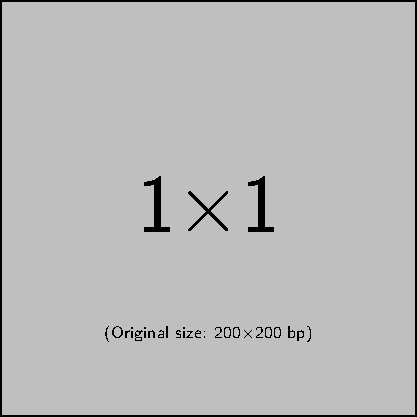
\includegraphics[width=.4\hsize]{figure/example-image-pdf.pdf}
   \caption{A example of includeing single figure.}
\end{figure}

%% 図の入れ方
\begin{figure}[t]
   % figure は t を指定する
   \centering
   % 横幅の 0.45 倍の minipage を 2x2 に配置
   %  [minipage][minipage]
   %  [1emの縦スペース]
   %  [minipage][minipage]
   \begin{minipage}{.45\hsize}
      \centering
      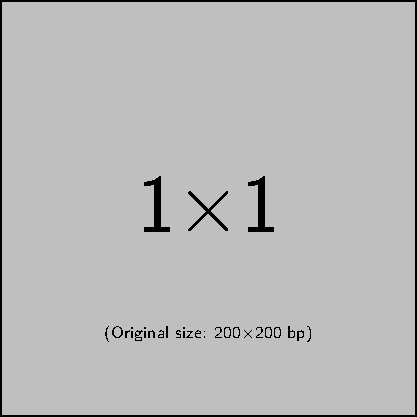
\includegraphics[width=.8\hsize]{figure/example-image-pdf.pdf}%
      \subcaption{Example Image A}
   \end{minipage}
   \begin{minipage}{.45\hsize}
      \centering
      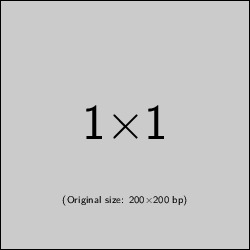
\includegraphics[width=.8\hsize]{figure/example-image-jpg.jpg}%
      \subcaption{Example Image B}
   \end{minipage}
   \\\vspace{1em}
   \begin{minipage}{.45\hsize}
      \centering
      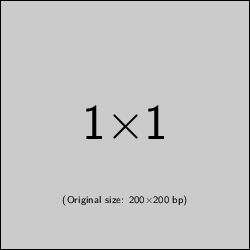
\includegraphics[width=.8\hsize]{figure/example-image-png.png}%
      \subcaption{Example Image C}
   \end{minipage}
   \begin{minipage}{.45\hsize}
      \centering
      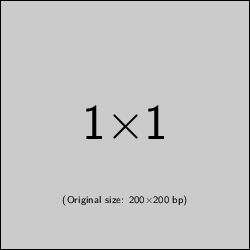
\includegraphics[width=.8\hsize]{figure/example-image-png.png}%
      \subcaption{Example Image D}
   \end{minipage}
   \caption{An Example of a Figure}
\end{figure}

%% 表の入れ方
\begin{table}[t]
   \centering
   %% 行間を 1.2 倍に広げる
   \renewcommand{\arraystretch}{1.2}
   \caption{An Example of a Table}
   \label{Tbl:Example}
   % 収まりきらないことが多いと思うので文字を小さくする
   % \footnotesize < \small < \normalsize (指定なし)
   \footnotesize
   %
   \begin{tabular}{c|c|c|c|c|c|c}
\hline\hline
        & \multicolumn{6}{c}{Number of Occurences} \\\cline{2-7}
        & 0 & 1 & 2 & 3 & 4 & 5 and more \\\hline
Scheme 1&\texttt{10}&\texttt{11} &\multicolumn{4}{c}{\scriptsize Flag 0} \\\hline
Scheme 2&\texttt{10}&\texttt{110}&\texttt{111} &\multicolumn{3}{c}{\scriptsize Flag 0}\\\hline
Scheme 3&\texttt{10}&\texttt{110}&\texttt{1110}&\texttt{1111} &\multicolumn{2}{c}{\scriptsize Flag 0} \\\hline
Scheme 4&\texttt{10}&\texttt{110}&\texttt{1110}&\texttt{11110}&\texttt{11111}&{\scriptsize Flag 0}\\\hline
\hline
   \end{tabular}
\end{table}

%% 段組にわたる図の入れ方
\begin{figure*}[t]
   \centering 
   % 幅 0.3\hsize の minipage を 3 つ横に並べる
   %    [minipage][minipage][minipage]
   \begin{minipage}[b]{.3\hsize}
      \centering
      
\includegraphics[width=.8\hsize]{figure/example-image-a.pdf} %
      \subcaption{Example Image A}
      \label{Fig:Example:A}
   \end{minipage}
   \begin{minipage}[b]{.3\hsize}
      \centering
      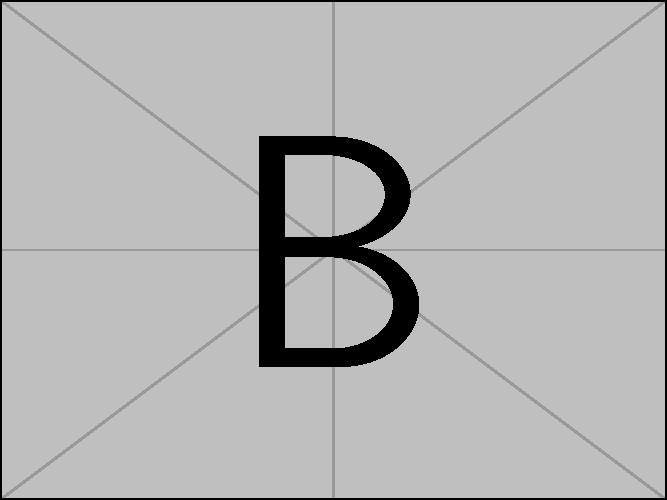
\includegraphics[width=.8\hsize]{figure/example-image-b.pdf} %
      \subcaption{Example Image B}
      \label{Fig:Example:B}
   \end{minipage}
   \begin{minipage}[b]{.3\hsize}
      \centering
      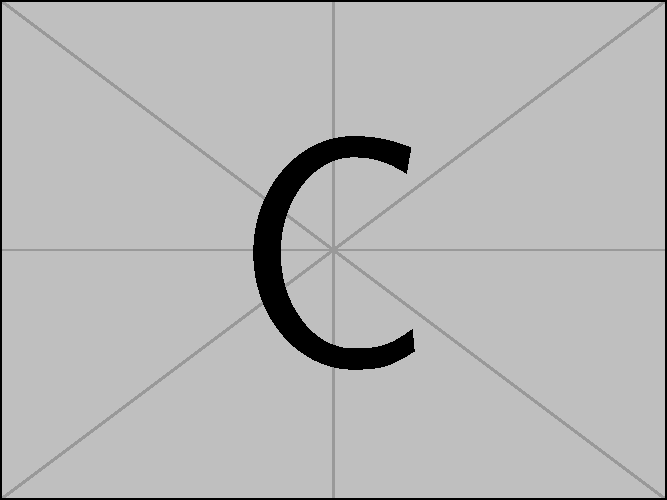
\includegraphics[width=.8\hsize]{figure/example-image-c.pdf} %
      \subcaption{Example Image C}
      \label{Fig:Example:C}
   \end{minipage}
   \caption{An Example of a Figure}
   \label{Fig:Example}
\end{figure*}

\section{An Example of Floating Algorithm}
\lipsum[5-6]

%% アルゴリズム図を入れる方法
%% algorithmic マークアップの書き方は以下を参照
%%   http://mirrors.ctan.org/macros/latex/contrib/algorithms/algorithms.pdf
\begin{algorithm}[t]
   \caption{An Example of an Algorithm}
   \begin{algorithmic}[1]
      \REQUIRE $n\geq0$
      \ENSURE $y=x^n$
      \STATE $S\leftarrow0$
      \IF{Condition}
         \STATE Do something.
      \ELSE
         \STATE Do something.
      \ENDIF
      \FOR{$i=0$ \TO $10$}
         \STATE Carry out some processing.
      \ENDFOR
      \RETURN $S$
   \end{algorithmic}
\end{algorithm}


%---------------------------------------------------------
% \balance コマンドを入れて最終ページの段組を揃える.
% 場所によってはうまく動作しないので適宜場所を調整する 
%  ・\bibliography の直前
%  ・Conclusion の節の直前
% など
\balance
%---------------------------------------------------------

\section{References}
\label{sec:ref}

List and number all bibliographical references at the end of the
paper. The references can be numbered in alphabetic order or in
order of appearance in the document. When referring to them in
the text, type the corresponding reference number in square
brackets as shown at the end of this sentence \cite{Example-Proceedings,Example-Article}.
An additional final page (the fifth page, in most cases) is allowed,
but must contain only references to the prior literature.

\section{Conclusion}
\lipsum[4]

%% 謝辞は IEEE Conference では入れない
%\section*{Acknowledgment}

%% 参考文献リスト
%% 参考文献のみのページにする場合は適宜 \newpage を入れてください
%\newpage
\bibliography{cites}

\end{document}
